\documentclass{article}


%
% Hyphenation etc...
%
\usepackage{ifxetex}
\ifxetex{}
  \usepackage{fontspec}
  \usepackage{csquotes}
  \usepackage{polyglossia}
  \setmainlanguage[variant=british]{english}
\else
  \usepackage[T1]{fontenc}
  \usepackage[utf8]{inputenc}
  \usepackage[UKenglish, english]{babel}
  \usepackage{lmodern}
\fi

%
% Colours
\usepackage[table, dvipsnames]{xcolor}

%
% Math
\usepackage{amsmath,amsfonts,amssymb,amsthm}
\usepackage{mathtools}
\usepackage{commath}  % derivatives, differentials
\usepackage{bm}  % bold math

%
% Hyper-links
\usepackage{hyperref}
\hypersetup{colorlinks,
            linkcolor={red!50!black},
            citecolor={blue!50!black},
            urlcolor={blue!80!black}}

%
% TODO
\usepackage[textsize=small]{todonotes}
\newcommand{\jr}[1]{\todo[author=JR, color=OliveGreen!20]{#1}}



%
% General document formatting
%
\usepackage{url}
\usepackage{xcolor}
\usepackage{graphicx}
\usepackage{booktabs}
\usepackage[printonlyused, withpage]{acronym}
% \usepackage[margin=0.7in]{geometry}
% \usepackage[parfill]{parskip}
% \usepackage[utf8]{inputenc}  % Not needed under xelatex


%
% Related to math
%
\usepackage{amsmath,amssymb,amsfonts,amsthm}


%
% Bibliography
%
\usepackage[
  backend=biber,
  doi=false,
  isbn=false,
  url=false,
  natbib=true]{biblatex}
\bibliography{CAGI5-reg-sat} % or
% \addbibresource{<database>.<extension>}


%
% Authorship and title
%
\usepackage{authblk}

\author[1]{Alex Hawkins-Hooker}
\author[1]{Henry Kenlay}
\author[1, 2]{John E. Reid}
\affil[1]{\footnotesize MRC Biostatistics Unit, University of Cambridge, Cambridge, UK}
\affil[2]{\footnotesize Alan Turing Institute, British Library, London, UK}

\title{A method for the CAGI 5 regulation saturation challenge}


\acrodef{CAGI}{Critical Assessment of Genome Interpretation}
\acrodef{SNV}{Single-Nucleotide Variant}
\acrodef{GWAS}{Genome-Wide Association Study}
\acrodefplural{GWAS}{Genome-Wide Association Studies}
\acrodef{MPRA}{Massively Parallel Reporter Assay}
\acrodef{eQTL}{Expression Quantitative Trait Locus}
\acrodef{ROC}{Receiver Operating Characteristic}
\acrodef{PR}{Precision-Recall}
\acrodef{AUROC}{Area Under the ROC curve}
\acrodef{AUPRC}{Area Under the Precision-Recall Curve}



\begin{document}

\maketitle


\todo[inline]{Any suggestions for catchy names for our method (acronyms or otherwise)?}


\section*{Introduction}

\subsection*{Biological context}

\acp{GWAS} have associated many \acp{SNV} with human traits and diseases.
Unfortunately several issues hinder the translation of this knowledge into an
understanding of the underlying biology and also into effective treatments of
disease.  First, linkage disequilibrium of neighbouring \acp{SNV} hinders
identification of the causal \acp{SNV}. Second, the majority of these \acp{SNV}
are in loci that do not code for proteins. The prevalent assumption is that the
causal mechanism is misregulation of gene expression. That is the regions they
occupy are important for the regulation of gene expression and this function is
disrupted by the \acp{SNV}.  However our understanding of how variation in
non-coding loci affects cellular function is relatively limited. 

To move from identification of disease-associated \acp{SNV} to potential
treatments the causal \acp{SNV} and their mechanisms must be identified.
\ac{eQTL} assays are suitable for fine-mapping the causal \acp{SNV} and can
associate underlying biological mechanisms with \acp{SNV} in linkage
disequilibrium.  However linkage hinders the statistical power of these assays
to identify the causal \ac{SNV}.

The genomic sequences of regulatory elements are assumed to encode most or all
of their function.  Methods that could predict \ac{SNV} effects on gene
expression based on sequence alone would help overcome the above mentioned
issues with linkage disequilibrium.

\acp{MPRA} are high-throughput assays to investigate internals of regulatory
elements.  \todo[inline]{Describe protocol.}

We describe our method to estimate \ac{SNV} effect sizes, trained on \ac{MPRA} data.
\ac{CAGI} 5 challenge.


\subsection*{Existing/similar methods}


\subsection*{Data}

17,500 \acp{SNV} in five enhancers and nine promoters (collectively \emph{regulatory
elements}) were assayed in a saturation mutagenesis \ac{MPRA}. A linear
regression model was fit to the data. This resulted in a \texttt{Confidence}
score (a monotonic function of the associated $p$-value) and \texttt{Value}
score for each \ac{SNV}\@. Briefly, the \texttt{Confidence} represents how sure we
are that the \ac{SNV} has an effect on gene expression and the \texttt{Value}
represents the direction and magnitude (positive for activating, negative for
repressing) of the effect (see Figures~\ref{fig:conf-value}
and~\ref{fig:training-sort1}). The SNVs were classified into three classes: if
the \texttt{Confidence} is less than $.1$, the \texttt{Direction} is 0;
otherwise the \texttt{Direction} is 1 (resp. -1) if \texttt{Value} $\ge 0$
(resp. $< 0$).

\begin{figure}[ht]
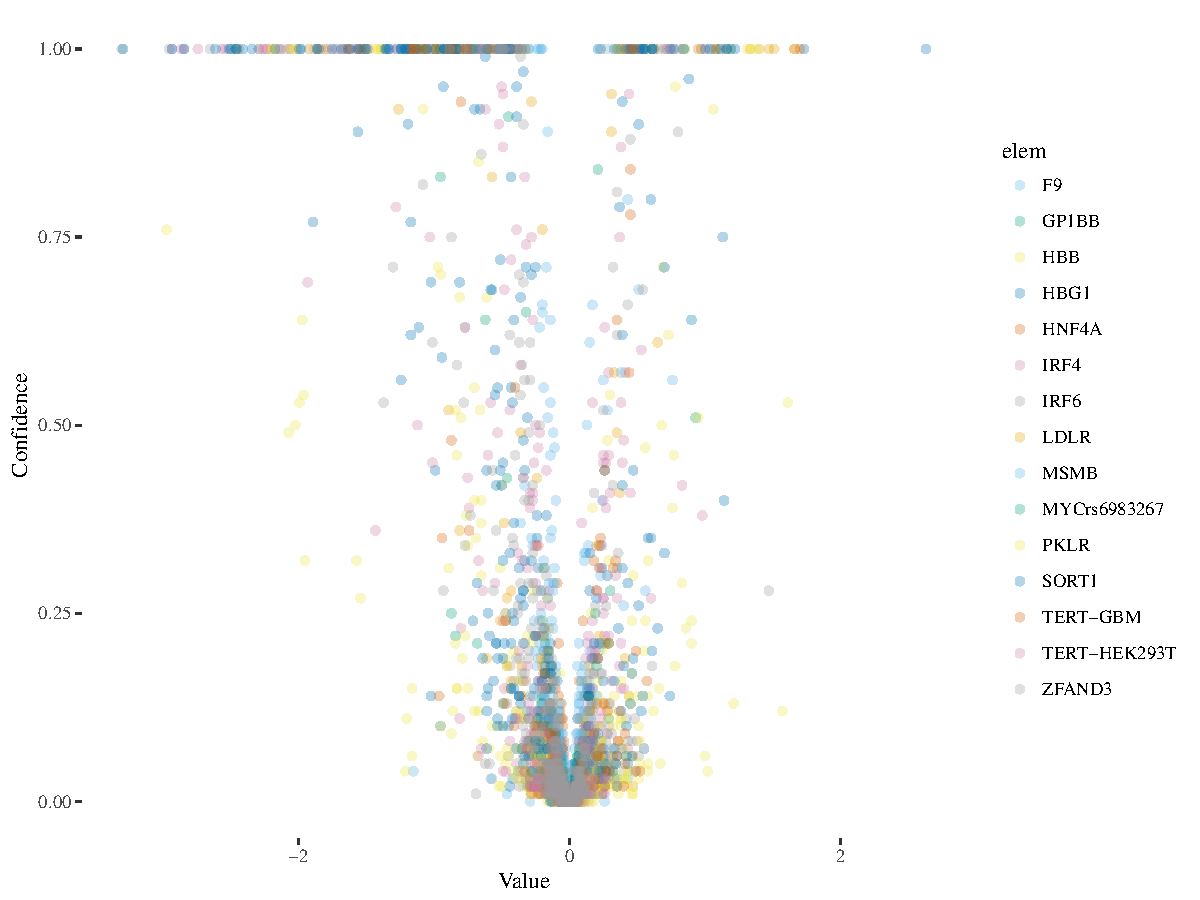
\includegraphics[width=\textwidth]{fig-conf-value-scatter}
\caption{Scatter plot of the confidence and value scores in the training data coloured
by regulatory element and cell line.}
\label{fig:conf-value}
\end{figure}

\begin{figure}[ht]
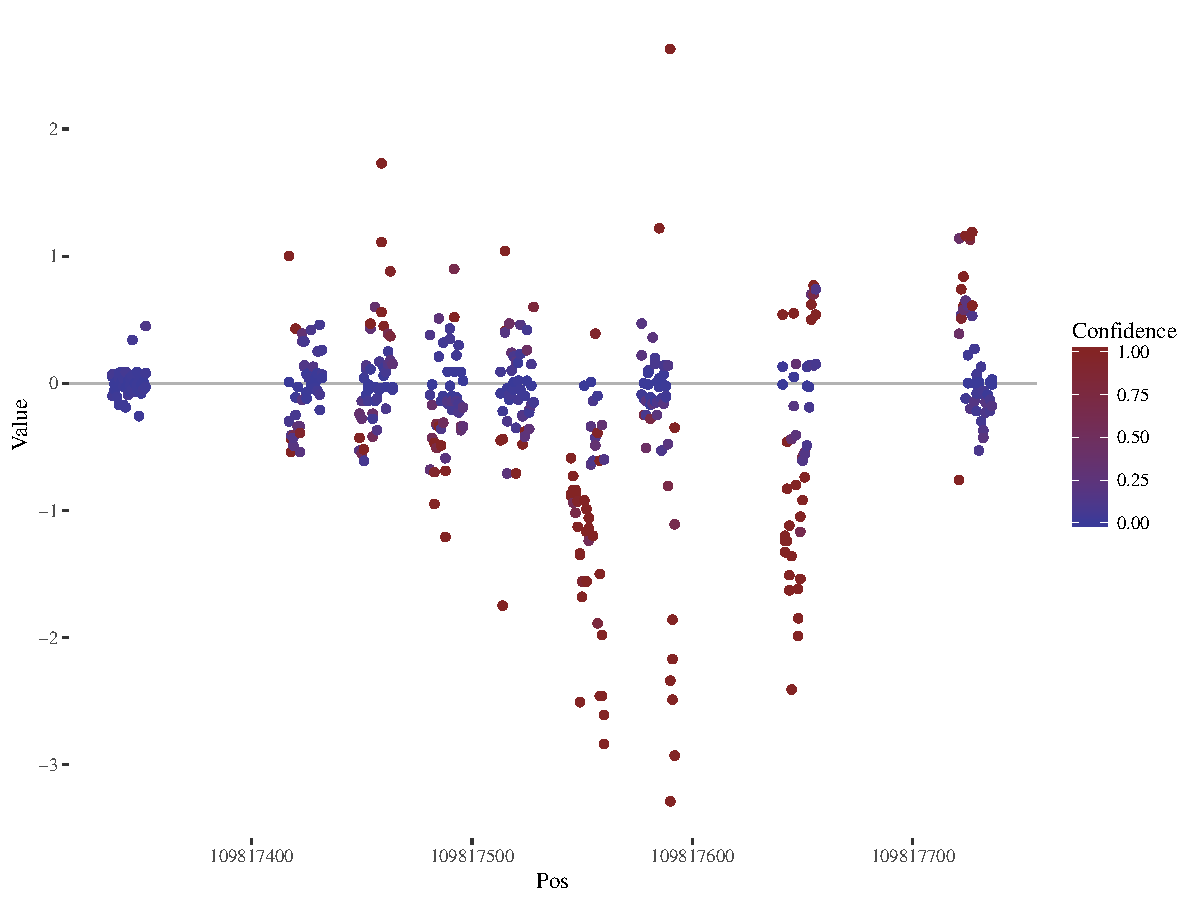
\includegraphics[width=\textwidth]{fig-value-conf-SORT1}
\caption{Training data for the SORT1 regulatory element.}
\label{fig:training-sort1}
\end{figure}

One regulatory element, \texttt{TERT}, was assayed in two cell lines. We
distinguish these experiments by \texttt{TERT-GBM} and \texttt{TERT-HEK293T}.


\subsection*{Prediction task}

The data was split 25\%--75\% into training and test data. Note that the
training data was chosen to form contiguous chunks (see
Figure~\ref{fig:training-sort1}).  The challenge required the participating
teams to enter a prediction for each \ac{SNV} in the test data. Each prediction
consisted of:
\begin{itemize}
  \item A categorical prediction of the \texttt{Direction} of the effect (-1, 0 or 1).
  \item The probability of correctly assigning the predicted \texttt{Direction},
    that is a measure of confidence in the prediction.
  \item A prediction of the \texttt{Confidence}.
  \item The standard error of the predicted \texttt{Confidence}.
\end{itemize}
The assessment metrics were loosely hinted at in the challenge description
but were not well-defined.


\section*{Methods}

We were inspired by Zeng et al.'s winning
method~\cite{ZengAccurateeQTLprioritization2017} from the CAGI~4
challenge~\citep{KreimerPredictinggeneexpression2017}.


\subsection*{Features}

We tested different types of feature to assess their predictive power.


\subsubsection*{Conservation}

We used phyloP~\cite{PollardDetectionnonneutralsubstitution2010},
phastCons~\cite{SiepelEvolutionarilyconservedelements2005}, GerpN
and GerpRS~\cite{CooperDistributionintensityconstraint2005} base-pair
resolved conservation scores.

Downloaded from UCSC~\cite{KuhnUCSCgenomebrowser2013}? \jr{AHH\@: can you check
where this came from?}


\subsubsection*{DNase hypersensitivity}

For each regulatory element we identified the closest matching
ENCODE~\cite{DunhamintegratedencyclopediaDNA2012} cell type for which there is
a DNase-hypersensitivity track (see Table~\ref{tab:encode-cell-types}). We
downloaded the tracks~\cite{RosenbloomENCODEDataUCSC2012} and created
41-dimensional features consisting of the signal at each base-pair flanked by
the signal at the bases 20bp on either side.

\begin{table}[htp]
\resizebox{\textwidth}{!} {\
\begin{tabular}{rll}
  \\
  challenge  & ENCODE    & UCSC track \\
  \toprule
  HepG2      & HepG2     & wgEncodeOpenChromDnaseHepg2BaseOverlapSignal \\
  HEL 92.1.7 & GM12878   & wgEncodeOpenChromDnaseGm12878BaseOverlapSignal \\
  HEK293T    & HEK293T   & wgEncodeOpenChromDnaseHek293tBaseOverlapSignal \\
  K562       & K562      & wgEncodeOpenChromDnaseK562BaseOverlapSignalV2 \\
  GBM        & Gliobla   & wgEncodeOpenChromDnaseGlioblaBaseOverlapSignal \\
  SK-MEL-28  & Colo829   & wgEncodeOpenChromDnaseColo829BaseOverlapSignal \\
  HaCaT      & NHEK      & wgEncodeOpenChromDnaseNhekBaseOverlapSignal \\
  MIN6       & PanIslets & wgEncodeOpenChromDnasePanisletsBaseOverlapSignal
\end{tabular}
}
\caption{The ENCODE cell lines that were identified as the closest
matches to the cell lines in the challenge. The corresponding UCSC track
names are also given.}
\label{tab:encode-cell-types}
\end{table}


\subsubsection*{DeepSea neural networks}

We trained several different neural network architectures on the genomic
prediction benchmark detailed in the original DeepSea
paper~\cite{ZhouPredictingeffectsnoncoding2015}. We evaluated these networks on
a region surrounding each variant twice, once with the reference allele and
once with the alternate allele. Features were generated as the difference in
activations between the two evaluations of internal and output layers of the
networks.

DanQ network~\cite{QuangDanQhybridconvolutional2016}.

\jr{AHH\@: We need some more details here. If I let you know which network features I used,
can you fill in the details of the network architectures and training?}


\subsubsection*{Region identity}

We one-hot encoded the identity of region to use as a feature.


\subsubsection*{Substitution}

We one-hot encoded the reference to alternate allele substitution as a feature.


\subsubsection*{Stacked predictions}

We generated features estimating the \texttt{Value} and \texttt{Confidence} by
fitting models to held out data. For the test SNVs, the held out data was the
training data. During cross-validation, features for the validation SNVs' were
estimated using the training folds as the held out data. We used the DeepSea
difference features, DNase features and conservation features to fit the
gradient boosting models estimating these generated features.

\begin{figure}
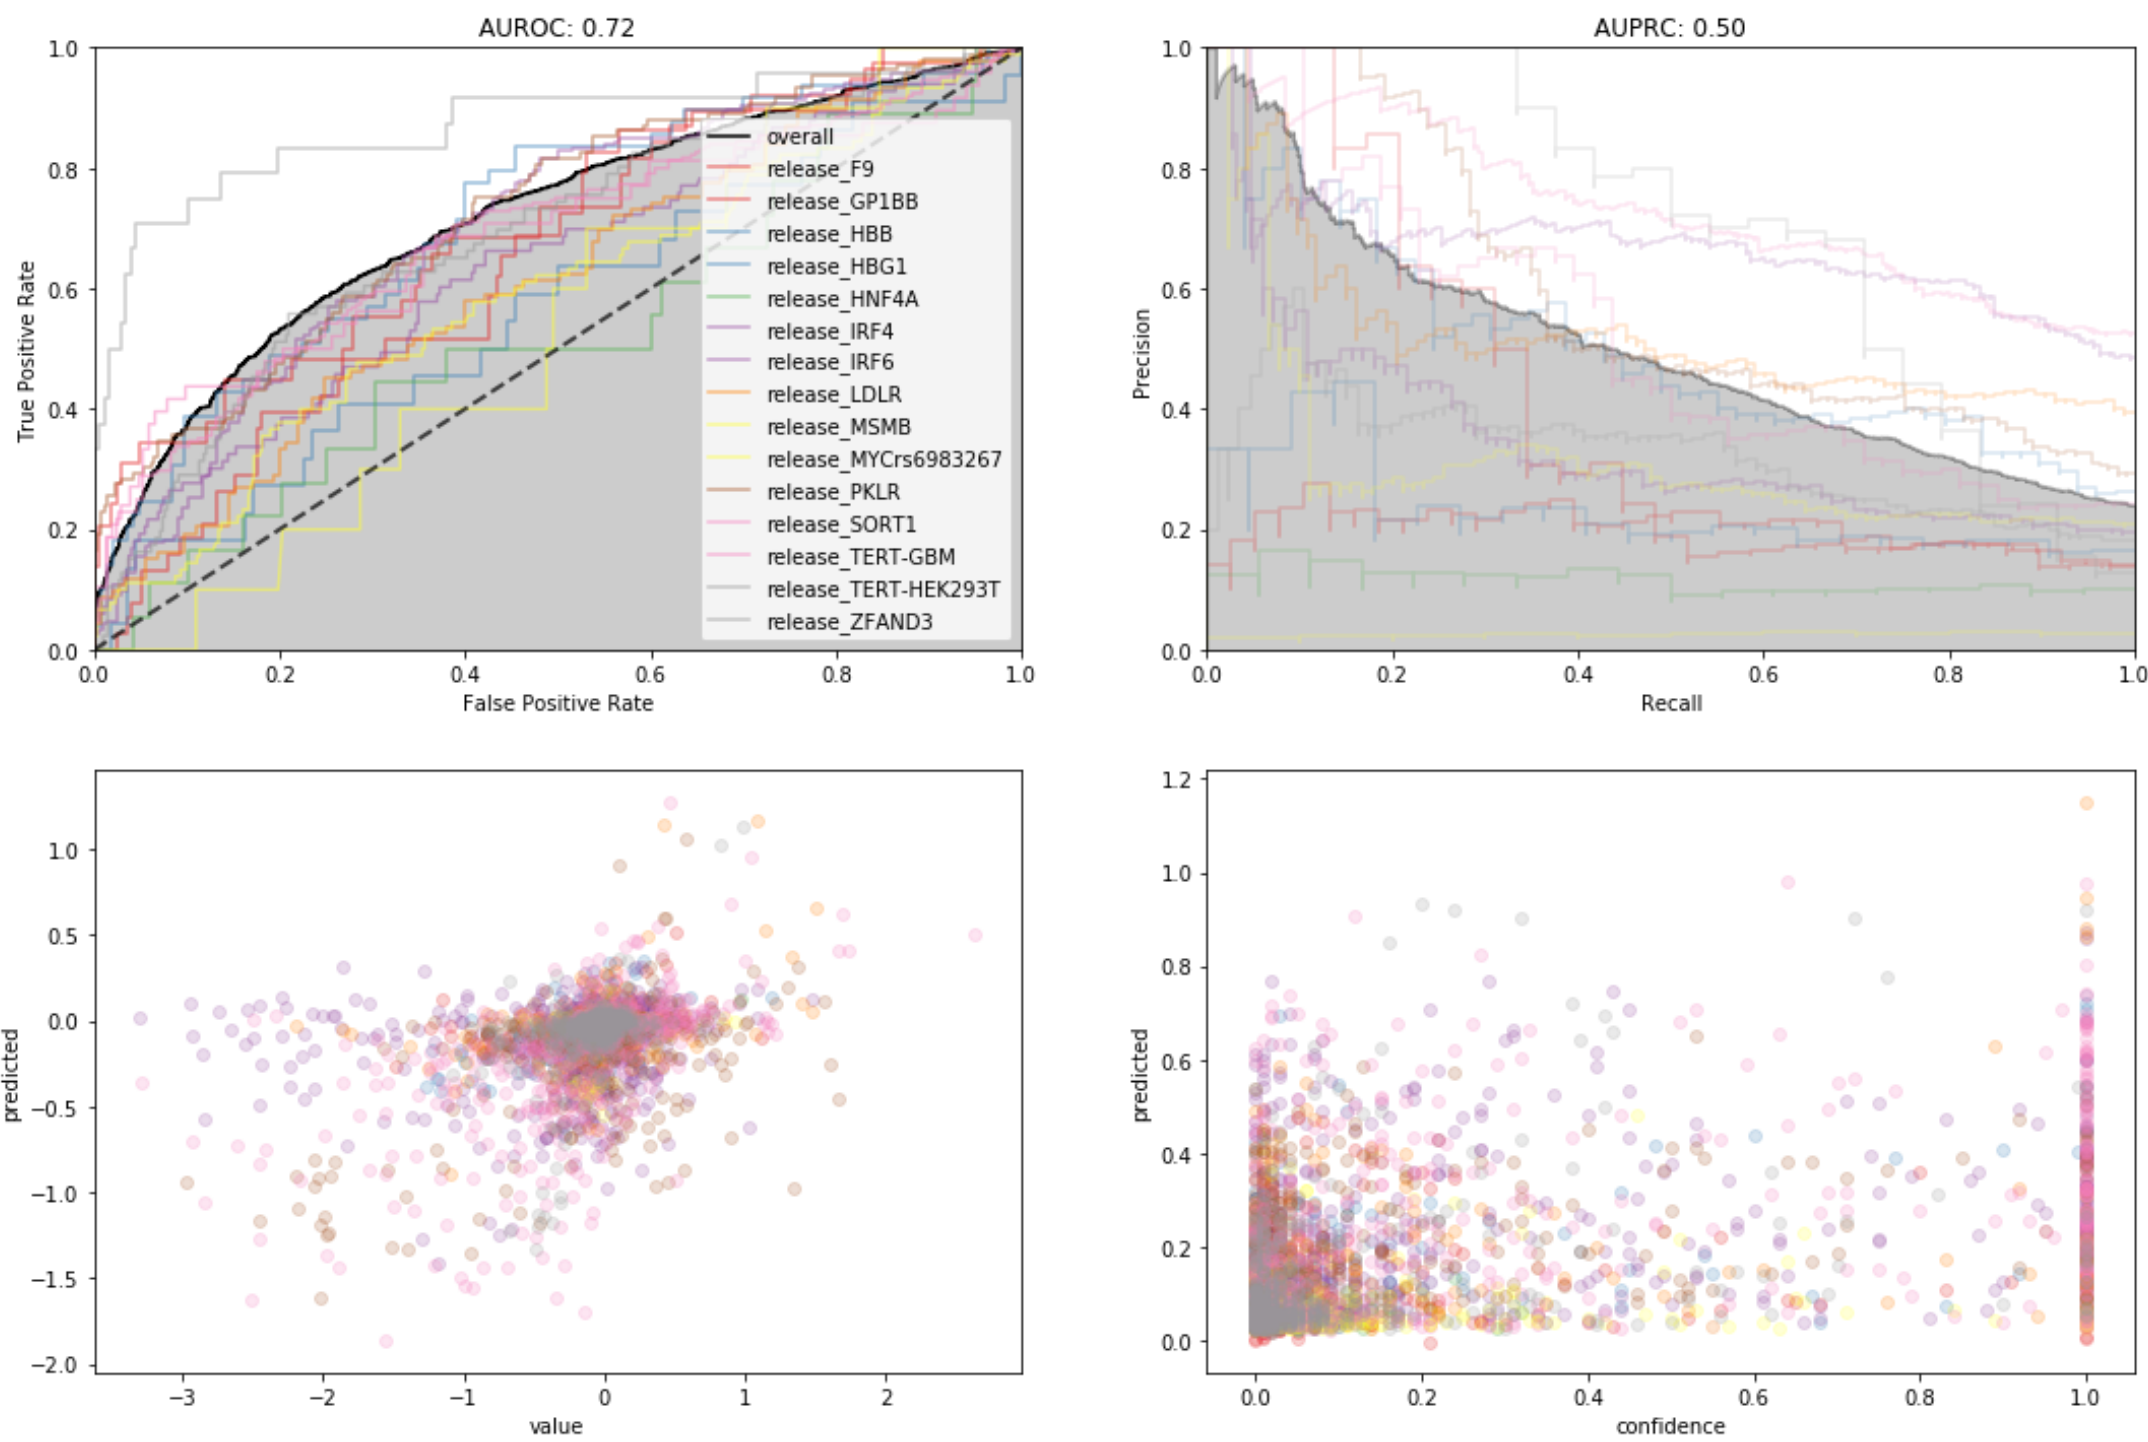
\includegraphics[width=\textwidth]{fig-stacking-x-validation}
\caption{Predictions used for stacking coloured by regulatory element.
  \emph{Top left}: Overall and regulatory element specific \ac{AUROC} for prediction
  of \texttt{Direction} using \texttt{Value}.
  \emph{Top right}: Overall and regulatory element specific \ac{AUPRC} for prediction
  of \texttt{Direction} using \texttt{Value}.
  \emph{Bottom left}: Predicted \texttt{Value} against actual \texttt{Value}.
  \emph{Bottom right}: Predicted \texttt{Confidence} against actual \texttt{Confidence}.
}
\label{fig:stacking}
\end{figure}


\subsection*{Inference}


\subsubsection*{Models}

We used three different gradient boosting algorithms:
XGBoost~\cite{ChenXGBoostScalableTree2016},
CatBoost~\cite{ProkhorenkovaCatBoostunbiasedboosting2017} and
LightGBM~\cite{KeLightGBMHighlyEfficient2017}. We used the gradient boosting
algorithms to regress the \texttt{Value} and \texttt{Confidence}, we also used
them as classifiers to predict the \texttt{Direction}. We tested different
subsets of features in a 5-fold cross-validation set up to identify the best
features.  Models were assessed by the cross-validated one against many
\ac{AUPRC}. We stacked models in that we used
the prediction of cross-validated regression models of the \texttt{Value} and
\texttt{Confidence} as features in the classification model for the
\texttt{Direction}.


\subsubsection*{Cross-validation}

We used a custom cross-validation configuration to investigate different models
and hyper-parameters.  The spatial dependence of the \texttt{Value} in each
regulatory element would clearly break the independence assumption in a naive
5-fold cross-validation.  Therefore we choose to perform 5-fold
cross-validation that retained spatial dependencies. Briefly, we defined chunks
as maximal contiguous regions in the training data for each regulatory element.

As the validation metrics for the challenge were ill-defined and the challenge
requires several predictions for each \ac{SNV} across 3 categorical outcomes, we
chose to use a simplified task to evaluate models and hyperparameters. We used
the absolute predicted \texttt{Value} as a predictor of the absolute
\texttt{Direction}.  This is a binary classification task and permits analysis
by \ac{ROC} and \ac{PR} curves. We used the \ac{AUPRC} as our primary
evaluation criteria when performing cross-validation. We also calculated the
\ac{AUROC} as a statistic of interest.

\todo[inline]{Precisely describe cross-validation scheme respecting structure of
training loci.}



\subsubsection*{Hyper-parameter Bayesian optimisation}

\todo[inline]{Describe Bayesian optimisation scheme}


\subsubsection*{Confidence standard error}

To estimate the standard error of the \texttt{Confidence} we trained an
ensemble of regression models and used the standard deviation of the
predictions to estimate the standard error.


\subsection*{Variable importance}

\todo[inline]{Discuss which features were important for prediction.}


\section*{Discussion}

\todo[inline]{Discuss why neural network features work so well}

\todo[inline]{Discuss how good results are}

\todo[inline]{Which regulatory elements were easier/harder?}

\todo[inline]{Future work/extensions}


\section*{Contributions}

HK, AHH and JR developed the deep convolutional neural network models of
genomic sequence. AHH and JR derived the features required for this
project. AHH and JR fit the gradient boosting machines. JR wrote the
manuscript.

All code to reproduce the submitted results is available in a git
repository~\url{git@bitbucket.org:alex-hh/cagimpra.git} which can be made
available on request.


\subsection*{Acknowledgements}

We are grateful to the organizers of the CAGI 5 experiment for running the
regulation saturation challenge. We thank Martin Kircher, Fumitaka Inoue,
Chenling Xiong, Beth Martin, Nadav Ahituv, and Jay Shendure for providing the
\ac{MPRA} data for this challenge. We also thank members of the MRC Biostatistics
Unit for providing helpful feedback on the method, in particular Elena
Vigorito, Lorenz Wernisch, Paul Newcombe, and Paul Kirk gave insightful
comments on parts of this work.


%
% Bibliography
%
\printbibliography{}

\end{document}
